\begin{enumerate}[label=\arabic*.,ref=\thesection.\theenumi]
\numberwithin{equation}{enumi}
\item The modulated signal is given by 
\begin{align}
	s(t) = \cos\brak{2\pi f_c t + \phi(t)}
\end{align}
where
\begin{align}
	\phi(t) = 2\pi k_f \int_{0}^{t}m(\tau)\,d\tau
\end{align}
List the various parameters in a table.
\\
\solution
\\
\begin{tabular}{|c|l|c|}
    \hline 
    \textbf{Parameter} & \textbf{Value} &\textbf{Description} \\ \hline
    $f_c $&  & Frequency of the carrier signal\\
    $\Delta{f}$ &  & Maximum Deviation \\  
    $K_{f}$ &  & Frequency sensitivity \\ 
    $\tau$ &  & Duplicate Variable\\ 
    t     &  & Sampling time\\  \hline
    \end{tabular}
    \\
\item Obtain a difference equation for computing $\phi(t)$.  Suggest a sampling rate.
\\
\solution
\item Plot the spectrum of the transmitted signal.
\\
\solution
The folowing code plots the spectrum of transmitted signal in \figref{fig:Trans}
\\
Executing
\begin{lstlisting}
python3 fm/tx/codes/tx_spec.py
\end{lstlisting}
\begin{figure}[H]
\centering	
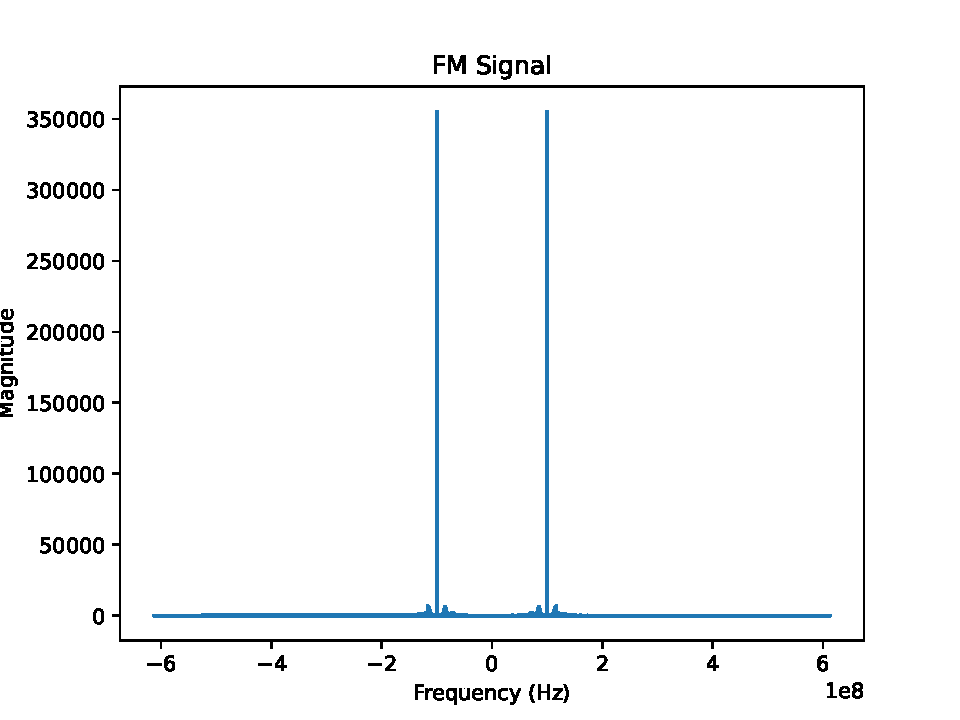
\includegraphics[width=\columnwidth]{fm/tx/figs/tx_spec.pdf} 
\caption{Plot of spectrum of transmitted signal.}
\label{fig:Trans}
\end{figure}

\item Compute the bandwidth of the transmitted signal.
\\
\solution
Executing
\begin{lstlisting}
python3 fm/tx/codes/tx_bw.py
\end{lstlisting}
gives the bandwidth of the message signal as 7190.695 Hz

\end{enumerate}
